\documentclass[letterpaper,10pt]{IEEEtran}
\usepackage{geometry}                % See geometry.pdf to learn the layout options. There are lots.
\geometry{letterpaper}                   % ... or a4paper or a5paper or ... 
%\geometry{landscape}                % Activate for for rotated page geometry
%\usepackage[parfill]{parskip}    % Activate to begin paragraphs with an empty line rather than an indent
\usepackage{graphicx}
\usepackage{amssymb}
\usepackage{epstopdf}
\usepackage{multicol}
\usepackage{tikz}
\usetikzlibrary{calc}
\usepackage{mathptmx}
\usepackage{amsmath}
\usepackage{algpseudocode}
\usepackage{url}
\newcommand{\BigO}[1]{\ensuremath{\operatorname{O}\bigl(#1\bigr)}}



\DeclareGraphicsExtensions{.pdf,.png,.jpg}
\usepackage{wrapfig}

% Spacing stuff
\usepackage[cm]{fullpage}
\addtolength{\voffset}{-.5in}
\setlength{\topmargin}{0pt}
\setlength\footskip{0pt}
\setlength{\parskip}{0cm}
%\setlength{\parindent}{1em}
%\usepackage[compact]{titlesec}
%\titlespacing{\section}{0pt}{2ex}{1ex}
%\titlespacing{\subsection}{5pt}{1ex}{2ex}
%\titlespacing{\subsubsection}{0pt}{0.5ex}{0ex}

\title{Sphere Project}
\author{
Donnie Smith (donnie.smith@gatech.edu) \\
Kyle Harrigan (kwharrigan@gatech.edu) 
}	
\date{October 25, 2012}                                           % Activate to display a given date or no date


\markboth{CS 6491 Fall 2012, Project 3}{}
\begin{document}

\bibliographystyle{IEEEtran}

\maketitle

 %\begin{abstract}
 
 
 %\end{abstract}
 
%\section{Introduction
%}
%\IEEEPARstart{I}{nitially} 

%\section{Results}

%\bibliography{cs6491}

\section{Adding Balls}
When the 'S' key is pressed, a ball is added to the scene.
In order to determine where the new ball D is placed, a line is drawn from the camera eyepoint to the location indicated by the mouse, and the first ball A that the new ball touches while moving along this line is determined.
The resting point for the new ball is determined by finding two additional balls B and C such that D is tangent to A, B, and C, and the angle between the original collision point and resting point is minimized.

\section{Creating the Mesh}
Every time a ball is added, the mesh enclosing the centers of the balls is recalculated.
The mesh is generated by shooting a roller ball R at the scene.
The radius of R is twice the maximum size of the constituent balls.
In the same manner as adding balls, a line to the scene is drawn, and the first point of intersection is determined.
The closest position in which the roller is tangent to the centers of three consituent balls is then determined.
Notice that for mesh generation, the roller is tangent to the centers, rather than the surfaces, of the constituent balls.

The roller ball is then rolled along each of the three faces of the first triangle.
For each edge, the next triangle is determined by finding the ball C that, combined with the two balls comprising the edge A and B, yields the smallest angle of rotation for the roller ball.
The triangle described by the centers of these three balls is added to the mesh.

The procedure is recursive: the roller rolls in three directions from the initial triangle, and in two directions from each subsequent triangle (excluding the direction from whence the roller came).
Added triangles are compared to triangles already in the mesh, and when a duplicate triangle is found, the recursion terminates.
\begin{figure}[!h]
\centering
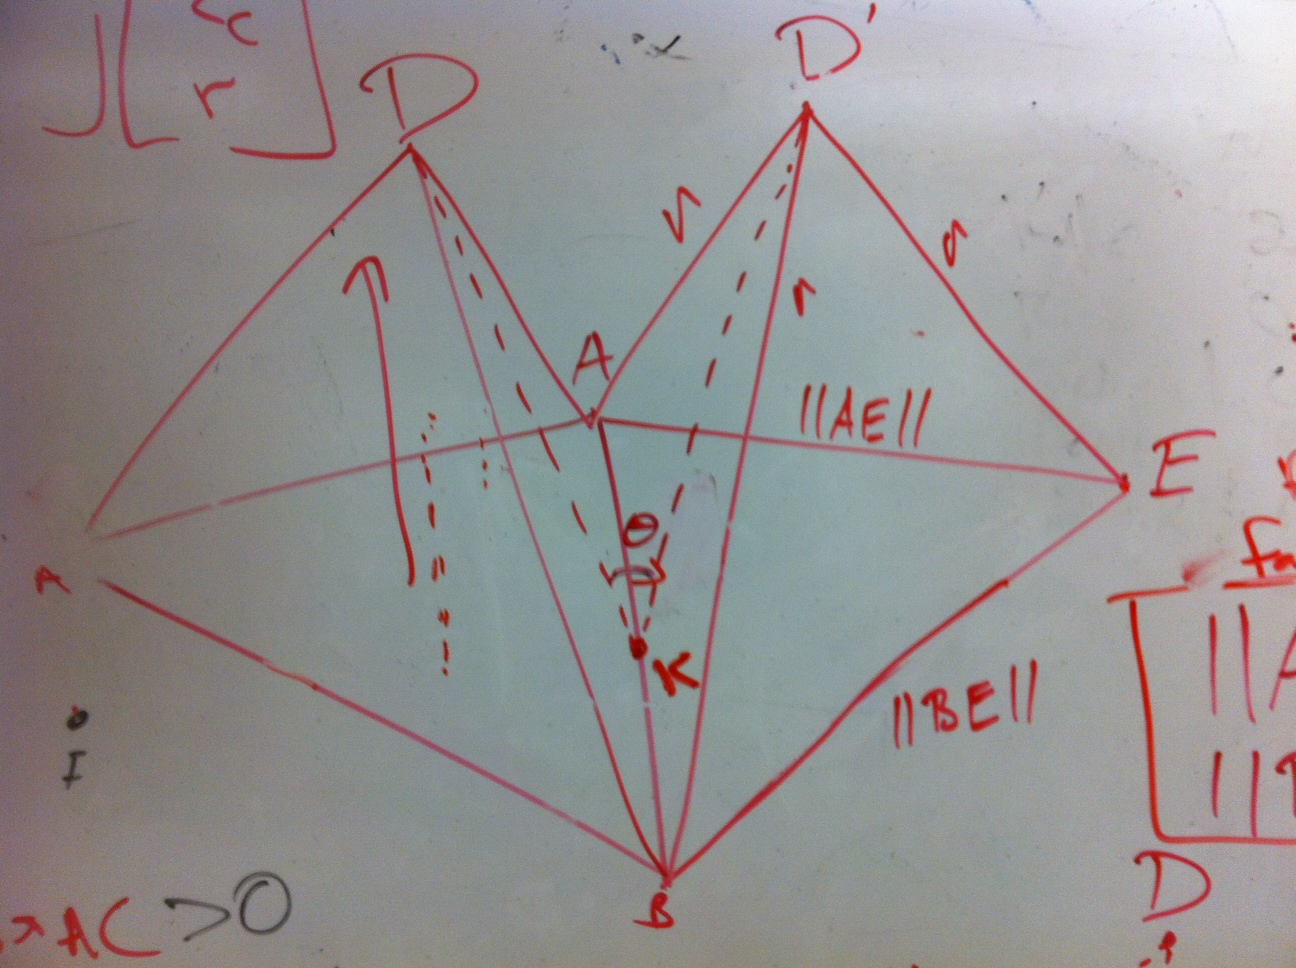
\includegraphics[width=1.75in]{main/data/angle}
\caption{Roller Ball Angle Calculation}
\label{fig_angle}
\end{figure}

\section{Algorithms}
The most significant algorithm work required determining the location of a ball D given the location of three balls A, B, C such that D is tangent to A, B, and C, or to the centers of those balls.
This problem can be reformulated as finding the location of one vertex of a tetrahedron in which the other three vertices, as well as the lengths of all edges, are known.
In this analogy, the vertices correspond to the centers of the balls, and the edge touching D are equal to the required distance between the centers (the sum of two radii if tangent to A, B, and C, or the radius of D if tangent to the centers).

The key to solving this problem lies in the observation that as the angle between triangle ABC and ABD changes, the projection of D onto the ABC plane traces a line perpendicular to AB.
A similar observation holds for the ACD triangle and AC.
Finding the intersection of these two lines yields the projection of D onto the ABC plane, D'.
D can be found by solving the right triangle AD'D to determine the length of DD'.
Adding a vector V of length $||DD'||$ and direction perpendicular to ABC yields D.
Since there are two directions perpendicular to ABC, there are two solutions to this problem.
In general, the one that minimizes some angle will be preferred.

This solution is outlined at http://www.had2know.com/academics/tetrahedron-volume-6-edges.html.

\section{Future Work}
A better canvas would make drawing easier.
One possibility is a plane on which balls can be placed on, or a choice between several starting configurations.
In addition, a toolbar style mode selection (Add Ball mode, Delete Ball mode) would make the application more user-friendly.

%\begin{IEEEbiography}[{\includegraphics[width=1in,height=1.25in,clip,keepaspectratio]{main/data/dsmith.png}}]{Donnie Smith} donnie.smith@gatech.edu
%\end{IEEEbiography}
%
%\begin{IEEEbiography}[{\includegraphics[width=1in,height=1.25in,clip,keepaspectratio]{main/data/kwharrigan.jpg}}]{Kyle Harrigan} kwharrigan@gatech.edu
%\end{IEEEbiography}
\end{document}
